\documentclass[a4paper,12pt]{article}

\usepackage[T2A]{fontenc}			
\usepackage[utf8]{inputenc}			
\usepackage[english,russian]{babel}	

\usepackage[
bookmarks=true, colorlinks=true, unicode=true,
urlcolor=black,linkcolor=black, anchorcolor=black,
citecolor=black, menucolor=black, filecolor=black,
]{hyperref}

\usepackage{color}
\usepackage{caption}
\DeclareCaptionFont{white}{\color{black}}
\DeclareCaptionFormat{listing}{\colorbox{white}{\parbox{\textwidth}{#1#2#3}}}
\captionsetup[lstlisting]{format=listing,labelfont=white,textfont=white}

\usepackage{amsmath,amsfonts,amssymb,amsthm,mathtools} 
\usepackage{wasysym}

\usepackage{graphicx}
%\usepackage[cache=false]{minted}
\usepackage{cmap}
\usepackage{indentfirst}

\usepackage{listings} 
\usepackage{fancyvrb}

\usepackage{geometry}
\geometry{left=2cm}
\geometry{right=1.5cm}
\geometry{top=1cm}
\geometry{bottom=2cm}

\setlength{\parindent}{5ex}
\setlength{\parskip}{0.5em}

\usepackage{pgfplots}
\usetikzlibrary{datavisualization}
\usetikzlibrary{datavisualization.formats.functions}

\begin{document}
	\lstset{ %
		language=C,                 % выбор языка для подсветки (здесь это С)
		basicstyle=\small\sffamily, % размер и начертание шрифта для подсветки кода
		numbers=left,               % где поставить нумерацию строк (слева\справа)
		numberstyle=\tiny,           % размер шрифта для номеров строк
		stepnumber=1,                   % размер шага между двумя номерами строк
		numbersep=5pt,                % как далеко отстоят номера строк от подсвечиваемого кода
		backgroundcolor=\color{white}, % цвет фона подсветки - используем \usepackage{color}
		showspaces=false,            % показывать или нет пробелы специальными отступами
		showstringspaces=false,      % показывать или нет пробелы в строках
		showtabs=false,             % показывать или нет табуляцию в строках
		frame=single,              % рисовать рамку вокруг кода
		tabsize=2,                 % размер табуляции по умолчанию равен 2 пробелам
		captionpos=t,              % позиция заголовка вверху [t] или внизу [b] 
		breaklines=true,           % автоматически переносить строки (да\нет)
		breakatwhitespace=false, % переносить строки только если есть пробел
		escapeinside={\%*}{*)}   % если нужно добавить комментарии в коде
	}
	
	% Титульный лист
	\begin{figure}[h!]
		\begin{center}
			{
\includegraphics[scale = 0.4]{titul.jpg}}
			\label{titul}
		\end{center}
	\end{figure}
	
	\vspace*{15mm} 
	
	\huge
	\begin{center}
		Дисциплина: <<Функциональное и логическое программирование>>
	\end{center}
	\vspace*{15mm} 	
	
	\begin{center}
		Лабораторная работа №1
	\end{center}
	
	\vspace*{15mm} 	
	
	\large
	\begin{flushright}
		Студент: Левушкин И. К. \\
		Группа: ИУ7-62Б \\
		Преподаватели: Толпинская Н. Б., \\ Строганов Ю. В. \\
	\end{flushright}
	
	\vspace*{30mm}
	\begin{center}
		Москва, 2020 г.  
	\end{center}
	\thispagestyle{empty}
	
	
	\newpage
	
	\section{Представить списки в виде списочных ячеек}
	
	\subsection{'(open close halph)}
	
	\begin{figure}[h!]
		\begin{center}
			{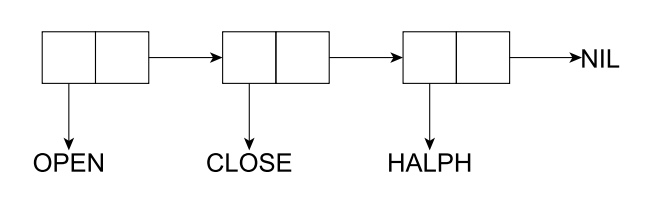
\includegraphics[scale = 0.4]{first.jpg}}
			\label{ris:1}
		\end{center}
	\end{figure}
	
	\subsection{'((open1) (close2) (halph3))}
	
	\begin{figure}[h!]
		\begin{center}
			{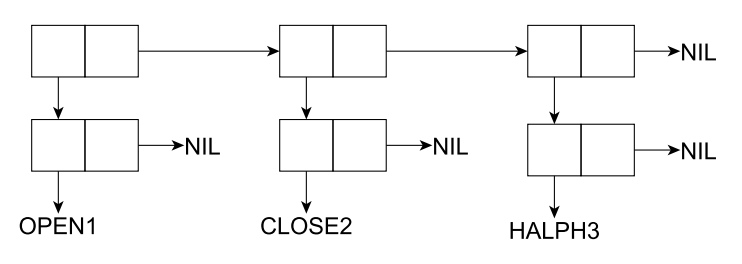
\includegraphics[scale = 0.4]{second.jpg}}
			\label{ris:2}
		\end{center}
	\end{figure}
	
	\subsection{'((one) for all (and (me (for you))))}
	
	\begin{figure}[h!]
		\begin{center}
			{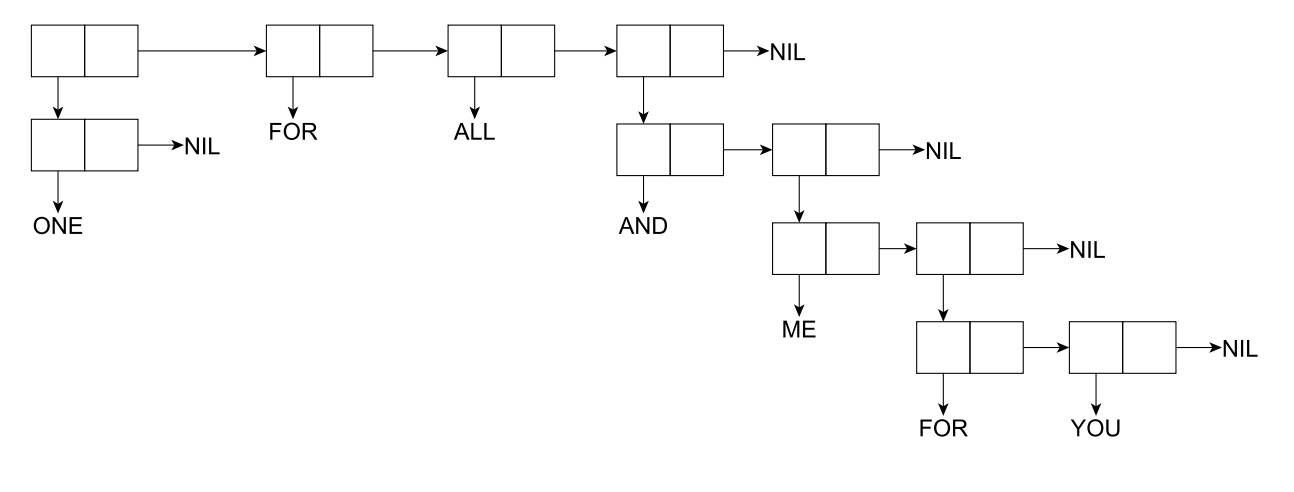
\includegraphics[scale = 0.4]{third.jpg}}
			\label{ris:3}
		\end{center}
	\end{figure}

\newpage
	
	\subsection{'((TOOL) (call))}
	
	\begin{figure}[h!]
		\begin{center}
			{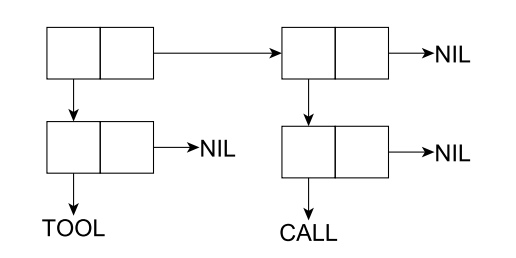
\includegraphics[scale = 0.4]{fourth.jpg}}
			\label{ris:4}
		\end{center}
	\end{figure}
	
	\subsection{'((TOOL1) ((call2)) ((sell)))}
	
	\begin{figure}[h!]
		\begin{center}
			{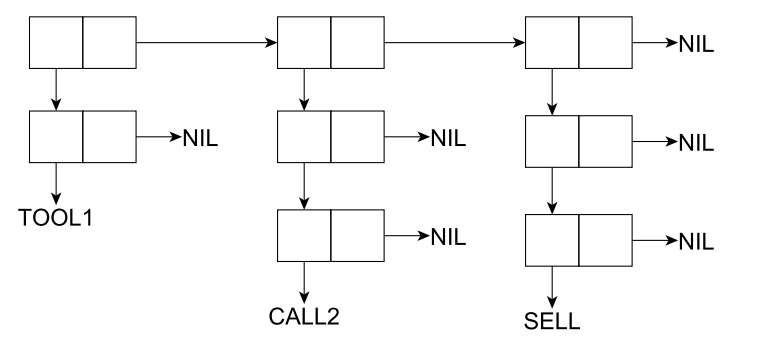
\includegraphics[scale = 0.4]{fifth.jpg}}
			\label{ris:5}
		\end{center}
	\end{figure}
	
	\subsection{'(((TOOL) (call)) ((sell)))}
	
	\begin{figure}[h!]
		\begin{center}
			{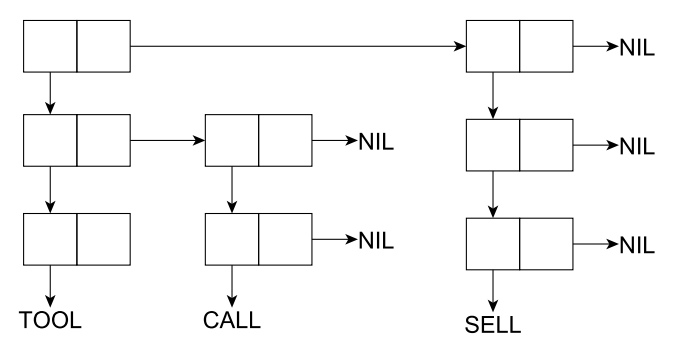
\includegraphics[scale = 0.4]{sixth.jpg}}
			\label{ris:6}
		\end{center}
	\end{figure}

\newpage
	
	\section{Используя только функции CAR и CDR, написать выражения, возвращающие необходимый элемент списка:}
	
	\subsection{второй}
	
	\begin{table} [h!]
		\begin{center}
			\begin{tabular}{|l|l|}
				\hline
				{\bf  Выражение} &    {\bf Результат} \\
				\hline
				{ (cadr '(a b c d e))}& b\\
				\hline
				{(cadr '((1 2) (3 4) (5 6)))}& (3 4)\\
				\hline
				{ (cadr '((one) for all (and (me))))}& for\\
				\hline
				{ cadr '(abc ((def) 1 y 3) (4 5) u v (z))}& ((def) 1 y 3)\\
				\hline
			\end{tabular}  
			\label{m1}
		\end{center}
	\end{table}
	
	\subsection{третий}
	
	\begin{table} [h!]
		\begin{center}
			\begin{tabular}{|l|l|}
				\hline
				{Выражение} &    {\bf Результат} \\
				\hline
				{(caddr '(a b c d e))}& c\\
				\hline
				{ (cadr '((1 2) (3 4) (5 6)))}& (5 6)\\
				\hline
				{ (cadr '((one) for all (and (me))))}& all\\
				\hline
				{ cadr '(abc ((def) 1 y 3) (4 5) u v (z))}& (4 5)\\
				\hline
			\end{tabular}  
			\label{m2}
		\end{center}
	\end{table}
	
	\subsection{четвертый}
	
	\begin{table} [h!]
		\begin{center}
			\begin{tabular}{|l|l|}
				\hline
				{Выражение} &    {\bf Результат} \\
				\hline
				{(cadddr '(a b c d e))}& d\\
				\hline
				{ (cadddr '((1 2) (3 4) (5 6)))}& Nil\\
				\hline
				{(cadddr '((one) for all (and (me))))}& (and (me))\\
				\hline
				{cadddr '(abc ((def) 1 y 3) (4 5) u v (z))}& u\\
				\hline
			\end{tabular}  
			\label{m3}
		\end{center}
	\end{table}
	
	\section*{Рекурсивное определение списка}
	
	Список является динамической структурой, может быть как пустым, так и непустым. Если он непустой, то должен иметь голову и хвост, который также представляется списком.
	
	\section*{Базовые принципы Lisp}
	
	\begin{enumerate}
		\item Условные высказывания
		\item Функциональный тип данных
		\item Рекурсия
		\item Динамическое типизирование
		\item Сборка мусора
		\item Программы, составленные из выражений
		\item Символьный тип
		\item Нотации для кода, использующего деревья символов и констант
		\item Постоянная целостность языка
	\end{enumerate}
	
	
\end{document}